%As an intrinsic quantum phenomena many particles have a non-zero spin component which we will name $\vec{S}$ and therefore they will have a spin intrinsic dipole moment $\vec{\mu}$ which is:

%\begin{align*}
%    \vec{\mu}^{(s)} &= \gamma \vec{S}\\
%\end{align*}

%We can note that $\gamma$ is an intrinsic quantity associated with fundamental particles which is defined by the relation $\gamma = g \frac{q}{2m}$, where $q$ is the electric charge of the particle, $m$ is the mass and $g$ is a proportionality constant defined for each particle. %Unsure of how accurate this is

\subsection{Resonance Condition: Larmor Frequency}

By starting out and modelling a simple particle in a static magnetic field ($\vec{B_o}$) we can represent the Hamiltonian as: $H_o = -\vec{\mu} \cdot \vec{B_o}$, where we define the magnetic moment as $\mu = g \frac{q}{2m} \vec{S}$. Here $q$ is charge, $m$ is mass, and $g$ as a proportionality constant (known as the $g$-factor). For any particle the $q$ and $m$ ratio will be unique, so we label this unique, identifying ratio the gyromagnetic ratio, $\gamma = g\frac{q}{2m}$. \\

Choosing the static field to be in the $\hat{z}$ axis, we can now state that:
\begin{align*}
    H_o &= - \gamma \vec{S} \vec{B_o}\\
        &= - \gamma \vec{S_z} B_o \label{H}\numberthis
\end{align*}

The $S_z$ component for the spin $\frac{1}{2}$ (proton/electron) is defined as: $S_z = \ket{\uparrow} \bra{\uparrow} - \ket{\downarrow} \bra{\downarrow}$. Solving this Hamiltonian, gives us two possible energy eigenvalues which correspond to two possible states of spin up ($\uparrow$) and spin down ($\downarrow$). Hence we will label the allowed energies as $E_\uparrow$ and $E_\downarrow$. 

\begin{align}
    & E_\uparrow = -\gamma \frac{\hbar}{2} B_o &
    & E_\downarrow = \gamma \frac{\hbar}{2} B_o
\end{align}

This means we can only have energy transitions of: $\Delta E  = E_\downarrow - E_\uparrow $. Translating this to a frequency we can state this photon absorption/emission frequency is:
\begin{align}
    \omega &= \frac{\Delta E}{\hbar} \nonumber \\
    \omega &= \frac{E_\downarrow - E_\uparrow}{\hbar}  \nonumber \\
    \omega &= \gamma B_o \tag{Larmor frequency}\label{Lfreq}
\end{align}

We can also find the \ref{Lfreq} classically by considering that if the particle is not aligned with our static magnetic field it will experience a torque defined as: $\vec{\tau} = \vec{\mu} \cdot \vec{B_o}$ which will lead to a procession about the axis of the static field. This frequency of procession is exactly $\omega$, the \ref{Lfreq}. \clearpage

\subsection{Perpendicular Magnetic Field: Rabi Oscillations}

The Hamiltonian in the energy basis is :
\begin{align}
    H_o = E_\uparrow \ket{\uparrow} \bra{\uparrow} + E_\downarrow \ket{\downarrow} \bra{\downarrow} \label{H_energy}
\end{align}

Creating a potential to induce transitions in the $xy$-plane and calling this potential $\vec{B_1}$ and allowing it to rotate at the \ref{Lfreq} gives us:
\begin{align*}
    V(t) &= -\vec{\mu} \cdot \vec{B_1}\\
    V(t) & = \gamma B_1 \frac{\hbar}{2} \big{(} e^{-i \omega t } \ket{\uparrow} \bra{\uparrow} + e^{i \omega t } \ket{\downarrow} \bra{\downarrow} \big{)}\\
\end{align*}

We now note that generally we can prove working in the Dirac Interaction picture gives:
\begin{align*}
   & i \hbar \frac{\partial}{\partial t} \ket{\psi (t)} = V(t) \ket{\psi (t)} \\[2em]
   \intertext{%It is also generally true that in energy basis that: } 
   }
   & \ket{\psi (t)} = \sum_n c_n \ket{n} & \ \\
    & H_o \ket{n} = E_n \ket{n}\\ 
    \intertext{Combining the above three equations we have that:} 
    &  i \hbar \frac{\partial}{\partial t} c_n (t) = \sum_m c_m V_{nm}(t) e^{i \omega_{nm} t}
\end{align*}

We note that $\omega_{nm}$ is the transition frequency which, for our originally stated particle, is the \ref{Lfreq}. We also note that plugging in our stated potential (Equation \ref{H}) gives us a single solution for $c_\uparrow$ and $c_\downarrow$ which is:
$c_\uparrow = c_\downarrow = \sqrt{1/2} \cdot c^{i \gamma B_1}$. So, the atoms will transition between $\ket{\uparrow} \text{ and } \ket{\downarrow}$ at a frequency of:
\begin{equation}
    \omega_R = \gamma \frac{B_1}{2} \tag{Rabi frequency} \label{Rfreq}
\end{equation}

This means that the additional magnetic field which is applied at the \ref{Lfreq} will create an oscillation between the two states at a rate of the \ref{Rfreq}.

\subsection{Nuclear Magnetization}

The bulk magnetic moment of a sample is the summation of magnetic moments, if we assume that the atoms have no orientation preference. Usually this discussed in the context of paramagnets, which are the summation of atomic-based electron distributions, but we note that this effect can also occur with nuclear magnetic moments as well. This summation of nuclear magnetic moments leads us to $\vec{M} = \vec{\mu} \left( C_\uparrow - C\downarrow \right)$, where $C_{\uparrow \downarrow}$ are the concentrations of up vs down spin states. \\

Due to the $B_o$ static magnetic field we have an energy difference of $\Delta E = 2 \mu B_o$ and hence the number of protons in the lower energy state ($\uparrow$) is slightly lesser leading to a measurably larger $C_\uparrow$ than $C_\downarrow$. This distribution is due to thermal effects.

\subsection{Pulsed NMR}
When a $B_1$ pulse for time $\tau$ is applied, the magnetization will be changed by an angle of $\theta = \omega_R \tau$. This is the azimuthial angle with the static electric field, as $\theta = 0$. This means that with a carefully timed pulse we can force the overall $\vec{M}$ from $+\hat{z}$ to any azimuthial angle.\\

We describe the pulses by the affect they cause on the direction of $\vec{M}$. Hence a pulse which brings $\vec{M}$ to the xy plane is described as a $\pi / 2$ or $90^\circ$ pulse, and a pulse which brings it to $-\hat{z}$ as a $\pi$ or $180^\circ$ pulse. Of course any angle being created is possible, but only $\pi/2$ or $\pi$ pulses will be discussed.

\subsection{Defining Time Constants}

After the application of a $\pi/2$ pulse, $\vec{M}$ will process about the $z$-axis on the $xy$-plane at a rate of $\omega$, the \ref{Lfreq}. If a coil is placed around the sample the processing magnetization will produce a magnetic field, inducing a voltage within the wire (the same used to create the pulse) due to Faraday's Law. This will induce: $V(t) = V_o sin(\omega t ) \text{ where } V_o = \omega k M_T$, $M_T$ is defined as the magnetization component in the $xy$-plane, and $k$ is a scaling factor of the coil based off of factors such as shape and size of the coil and other physically constant features. From this, we can note that $V_o \propto  M_T$ as $k$ and $\omega$ are constants of the experiment.\\

A typical signal suffers from decay, which can be modelled as $V(t) = V_o e^{-t/T} sin(\omega t)$. The exponential decay can be described with a constant $T$ -- which can be broken up into individual quantities arising from different physical effects. These effects occur in different axes and are therefore presented as $T^*_2$ and $T_1$.\\

$T_1$ is the so called ``spin lattice relaxation time'' and this is an effect describing the amount of time it takes for the sample to reach thermal equilibrium. This return is only achieved in the direction of the static field as it is the spins returning to thermal equilibrium (a return to alignment with $B_o$). The decays can occur from any position, but solely add to the $+\hat{z}$ component.\\

$T_2$ is known as the ``spin-spin relaxation time'' and is defined as the amount of time it takes for the spins of a system to move out of phase with each other due to the local internal magnetic fields, which are produced by neighbouring spins. These are originally in phase due to the $B_1$ pulsed field forcing them to be at the same $xy$ angle. Thus after a magnetization $\vec{M}$ is turned onto the $xy$ plane, the spins begin to de-phase, decreasing the net $\vec{M}$ and decaying the signal.

This de-phasing can also occur due to inhomogonities in the applied static field, which always occur. This effect is noted as $\frac{1}{T^B_2}$, but can also be proven to be dominated by a linear term in a paramegnet based NMR which can be represented as: $\frac{1}{T^B_2} = \gamma \Delta B_o$, where the $\Delta B_o$ are the deviations of the static field from the perfect field. The term $1/T^*_2$ is commonly used to represent $1/T^*_2 = 1/T_2 +  1/T^B_2$. These effects are logically grouped together as phase decoherence times only affect the magnetization in the $xy$-plane.\\

We also note that any Rabi shift of $\pi/2$ will cause these orthogonal components to interact with each other, and thermal decay can bring a $xy$ aligned atom into the static field direction.\\

These effects all combine to give us a signal in the $xy$-plane of  $V(t) = V_o e^{-t/T_2^*} sin(\omega t)$ as defined above. Which can be seen in Figure \ref{fig:FID}. We note that the envelope which the decay occurs in is called the ``free induction decay'' (FID).

\begin{figure}[H]
    \centering
    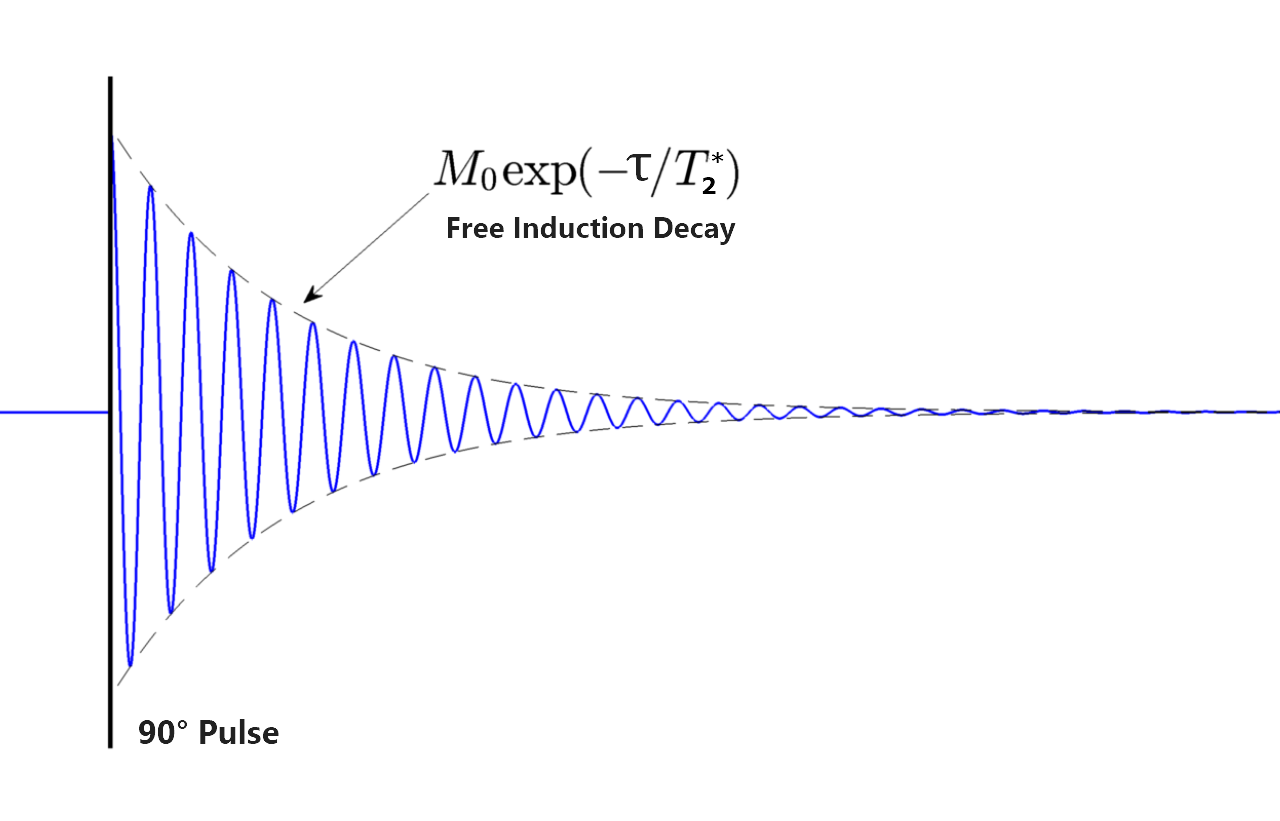
\includegraphics[width=.75\textwidth]{figures/FID_diagram_v2.png}
    \caption{Showing the signal which should be received from a $\pi/2$ pulse in an idealized simulation of an actual experiment.}
    \label{fig:FID}
\end{figure}

%We note that $\omega$, the \ref{Lfreq} for protons is 42.6 $MHz/T$ while the $1/T$ is on the order of 1 Hz. Therefore on a digital instrument, only one of these effects will be resolvable at a time.

